\documentclass{article}
\usepackage{color}
\usepackage[T1]{fontenc}
\usepackage[utf8]{inputenc}
\usepackage[francais]{babel}

\usepackage{graphicx}



\title{Rapport de projet 2048}
\author{Daubasse Bifert Gallardo}
\begin{document}
\maketitle
\tableofcontents
\textcolor{red}{\section{Présention du jeu 2048}}
Le but du jeu est de fusionner des nombres ensemble (puissance de deux) afin d'atteindre le nombre ultime '2048' et de gagner la partie.

L'aire du jeu 2048 est une grille de quatre lignes par quatre colonnes avec donc 16 cellules carrées. Chaque cellule peut être vide ou contenir un nombre. Au début du jeu, il y a deux carrés (également appelés « tuiles ») avec un chiffre '2' ou un '4' suivant votre chance à l'intérieur.
Lorsque vous parvenez à faire entrer en collision 2 briques avec le même numéro dedans, elles fusionnent en une seule nouvelle brique dont le numéro sera l'addition des deux nombres précédents : 2+2=4, 4+4=8, ... 1024+1024=2048 !
Pour déplacer les briques sur la grille, vous devez juste choisir une direction (haut, droite, bas ou gauche). Toutes les briques vont se déplacer dans la direction choisie, jusqu'à ce qu'elles fusionnent avec une brique de même valeur ou bien qu'elles soient bloquées par une brique avec un numéro différent. A chaque mouvement une tuile va aléatoirement apparaitre dans une case vide, cette tuile a une chance sur dix d'être égale a quatre sinon elle serra égale à deux.

Ici on utilisera simplement les quatres flèches directionnelles du clavier pour déplacer les briques.
\textcolor{red}{\section{Implémentation de la grille}}
\subsection{Fonctions simples}
\subsubsection{Valeur d'une tuile}
On donne les coordonnées et la grille afin de directement retourner la valeur de la tuile située dans cette grille et à ces coordonnées.
\subsubsection{Initialiser une tuile}
On donne les coordonnées et la grille afin de directement modifier la valeur de la tuile située dans cette grille et à ces coordonnées.
\subsubsection{Valeur du score}
On donne la grille et la valeur du pointeur du score de la grille est retournée.
\subsection{Structure}

Nous avons choisis d'implémenter la grille par un pointeur de pointeur d'entier pour la grille et d'un entier représentant le score.

Le pointeur nous sert à créer un tableau deux dimensions qui servira de grille, nous avons choisit la solution du pointeur car elle permet de facilement étendre notre grille a une taille supérieure à quatre.

Le tableau deux dimensions quant a lui nous semblait la solution la plus naturelle pour créer une grille.

C'est pourquoi nous n'avons pas implémenté la grille avec un tableau une dimension.


\subsection{Instanciation d'une grille}
Pour l'instanciation, dans la fonction new\_grid, d'une grille on alloue la mémoire pour une stucture de grille puis on initialise le score a zéro et ensuite on alloue le tableau deux dimensions en initialisant chacune des tuiles a zéro. On retourne ensuite la structure nouvellement crée.
\subsection{Suppression d'une grille}
Pour supprimer une instance de grille nous prenons en argument une stucture de grille et parcourons le tableau deux dimensions et nous libèront la mémoire allouer pour les pointeurs du pointeur tiles de notre structure puis on libère la mémoire prise par le pointeur tiles lui même et enfin on libère la mémoire de notre instance de grille.
\subsection{Copie d'une grille}
Pour copier une grille nous prenons en paramètre deux grille, src la source et dst la destination, nous parcourons ensuite le tableau deux dimension afin de copier chaque tuiles de src et de la placer dans la grille de dst une fois cela fait on copie le score de src et on le place dans le score de dst.
\subsection{Mouvement de la grille}
\subsubsection{Possibilité de mouvement}

Dans la fonction can\_move nous prenons en argument une grille et une direction.

L'idée ici est de se dire que si une tuile peut bouger alors l'ensemble de la grille le peut c'est pourquoi nous initialisons une variable booléenne a faux qui serra ensuite modifié, au fur et a mesure du parcours de notre tableau, si, en prenant une dirction donnée, deux tuiles consécutives sont égales mais différentes de zéro ou si la tuiles vérifié est égale a zéro, c'est à dire que l'on a un trou entre notre tuile et ce qu'il y a aprés que ce soit une autre tuiles, le bord de la grille ou encore un zéro.

On renvoie ensuite notre variable booléenne.

\subsubsection{Mouvement}

Pour le mouvement nous avons utilisée tois fonctions qui nous sont propre que sont array\_to\_grid, grid\_to\_array et compute\_array.\\

- Passage d'un tableau à une grille et d'une grille à un tableau:\par
Ces fonctions servent à transformer une grille en une ligne (tableau 1D de taille size) selon les parametres de position donnés, c'est à dire le paramètre x donnés en argument, et sans prendre en compte les zeros ensuite pour repasser d'une grille a un tableau on retransforme donc notre ligne 1D en grille en combalnt les tuiles vides par des zéros. En fonction du sens dans lequel nous voulons faire notre mouvement nous inversons ou non notre tableau, à l'aide de la foncton invert\_array, afin de traiter toute les directions de la même manière.
\\
\\
- Calcul du score:\par
La fonction compute\_array prend un tableau 1D et une taille, initialise un score à zéro et ensuite parcours ce tableau et pour chaque cases consécutive et identique du tableau les fussionent ajoutant leur somme à score qui est ensuite renvoyer à la fin de la fonction.
\\ \\

En utilisant ces fonction il est donc plus facile de faire le do\_move puisque que nous transformons notre grille en tableau 1D puis calculons notre nouvelle grille et le score dans ce tableau pour enfin remettre ce tableau dans notre grille.
\subsection{Ajout d'une tuile}
Ici nous créons un tableau deux dimensions et copiont les cases vides de notre grille prise en argument pour ensuite choisir hasard parmis ces cases celle que l'on placera à deux (ou quatre suivant le rand()). Nous choisisons de faire un rand entre 0 et 1000 car en effet le rand() rend des valeurs plus stable s'il est pris entre 0 et 1.
\subsection{Jouer un coup}
Jouer un coup reviens à vérifier que l'on peut bouger dans la direction demander par l'utilisateur et si c'est le cas faire le mouvement avec le do\_move et ajouter une tuile.
\subsection{Fin du jeu}
Nous détectons la fin du jeu quand aucune des directions n'est jouable, c'est à dire quand on ne peut plus bouger de tuile.
\textcolor{red}{\section{Test sur grid.c}}


  \subsection{Fonctions générales}
  Dans test\_grid.c nous avons essayer de vérifier le plus de code possible automatiquement.
  
  Pour nous aider nous avons crée une fonction result qui affiche, avec un code couleur, si le test est passer avec succés ou non.
  
  D'abord on teste que new\_grid crée bien une grille vide, on vérifie donc que chaque tuile est nulle.
  Ensuite on teste que la copy\_grid copie bien toute la grille c'est à dire le tableau deux dimension doit etre le même et le score lui aussi doit être copié.

  On crée donc deux grilles et vérifions à l'aide de la fonction equals du fichier grid\_utilities que chaque cases du tableau sont les même puis que les scores sont les même.
  Le test du score se fait juste par l'anticipation du score de la grille, on fixe donc deux cases et on vérifie que le score de la grille est bien le bon.

  Pour le test du can\_move nous créons deux grilles chacune avec une case occupée, une dans un coin et l'autre entourée par des cases vide.

  On vérifie ensuite que la première, celle avec la case dans le coin ne peut bougée que vers les directions opposées au coin quand à la deuxième, celle avec la case entourée de cases vides, doit pouvoir bougée dans tout les sens.
  
  Avec la deuxième grille nous testons notre do\_move en bougeant vers le haut puis vers la gauche et si on peut bougé dans toute les directions sauf le haut aprés avoir bougé en haut puis que l'on peut bouggé partout sauf vers le haut et la gauche après avoir bougé vers la gauche alors le test est passer avec succés.

  Enfin pour le add\_tile on fait autant de add\_tile que de case puis on vérifie que toute les cases sont occupées.
  
  \subsection{Fonction perso}
  
  Afin d'éviter tout bug innatendu nous avons décider de tester nos fonctions qui se trouvent dans grid\_utilities.

  On remplit donc un tableau de zéro à GRID\_SIZE (qui est la taille de toute nos grilles) et on l'inverse à l'aide de notre fonction, on vérifie alors que le tableau est bien inversé.

  Pour tester la fonction grid\_to\_array on remplit trois cases d'une grille de façon à avoir les même valeur que le tableau précédent dans les cases du haut, on applique notre fonction a la grille et on vérifie que nos tableaux sont identique.

  Pour le calcul de la nouvelle grille après mouvement on prend notre tableau de grille et l'on vérifie que ses valeurs sont bien les bonnes, c'està dire qu'elles doivent être rangée dans l'orde décroissant.

  Pour finir la fonction array\_to\_grid on prend notre grille que l'on avait au préalable transformé en tableau que l'on retransforme en grille et on vérifie ensuite que la valeur des tuiles du haut corresponde au tableau qui nous sert de référence dans les autres fonctions. Si ce sont les même la fonction ne contient pas de bug.
  
  \textcolor{red}{\section{Stratégie pour automatiser la résolution du jeu}}
  \subsection{Stratégie rapide (Moins de dix secondes de temps de calcul)}
  Au premier abord la stratégie qui semble la plus simple est celle dite du coin qui consiste a choisir une direction, si le mouvement est impossible changer de direction puis retourner à la première, si les deux premières sont bloqué passer à une troisième et de même pour la quatrième direction.

  Cette solution est très simple, ne demande aucun calcul et demande vraiment peu de temps à coder évidement elle est aussi trés peu fiable.

  Nous avons donc opter pour une stratégie qui commence comme celle du coin mais qui quand le choix de la troisième direction arrive choisis à l'aide de la fonction score la direction à prendre. La fonction score attribut à une grille un score ,rapidement calculé puisqu'il suffit d'enchainer huit parcours de grille.

  En effet à chaque parcours on pondère les valeurs de la grille ce qui nous aide à remplir un tableau dont on prendra l'indice de la valeur maximale.
  \subsection{Stratégie lente (Moins de deux minutes de temps de calcul)}

  Pour la strétégie longue nous avons opté pour une fonction récursive.

  Nous avions à la base penser à implémenter une structure d'arbre mais celà était trop fastidieux et au final n'avais pas beaucoup moins de calcul à réaliser comparé à notre fonction récursive.

  Nous avions donc eu l'idée de calculer chaque sous grille, c'est à dire les différentes grille possible en fonction des coups et des apparitions aléatoires des tuiles, de notre grille courante afin de choisir, parmis les quatres directions, la direction qui serait susceptible de donner la meilleure grille.
\\
  Pour choisir la meilleure grille nous attribuons encore une fois un score à ces grilles avec ces objectifs:
  \newline
  
  - Créer une grille progressive : plus précisément, il faut faire en sorte que la valeur des cases augmente ou descende quelle que soit la direction. Ainsi, 2 - 4 - 8 - 16 est acceptable, tout comme 32 - 8 - 4 - 2. Mais 2 - 8 - 2 - 16 ne l'est pas (à cause de la 3eme case).
  \\
  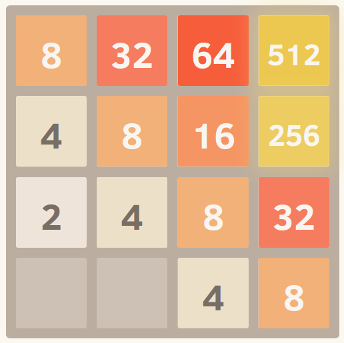
\includegraphics[scale=0.5]{../1.png}

Chaque mouvement doit donc être choisi en fonction du résultat qu'il va produire : la grille sera-t-elle plus progressive après le mouvement qu'avant ? Si oui, on s'oriente sur un bon score. Si non, le score sera mauvais. L'idée ici est qu'il faut placer les valeurs les plus hautes sur les extérieurs pour éviter qu'une valeur faible se retrouve coincée entre deux valeurs hautes et ne puisse être fusionnée.

- Gérer la régularité des cellules : pour pouvoir fusionner, les cases doivent comporter des valeurs identiques. Ainsi une suite 2 - 16 - 64 - 256 respecte la première règle (progressivité) mais aboutira à un échec car on ne pourra fusionner aucune case avec sa voisine.

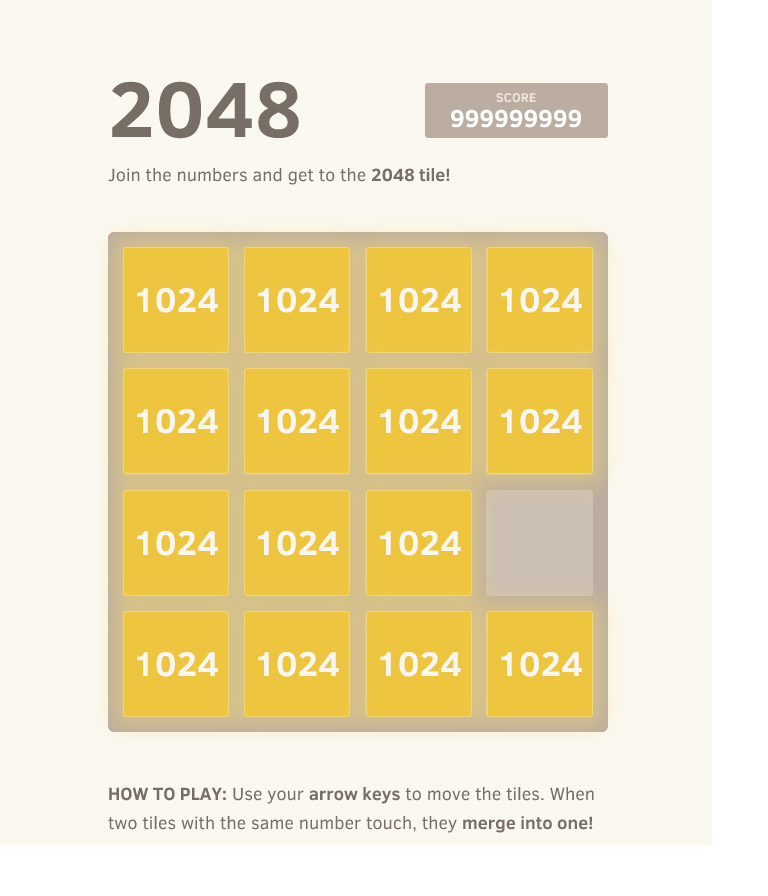
\includegraphics[scale=0.2]{../image.png}

Il faut donc respecter un second critère : la régularité. Et faire en sorte de ne pas avoir de rupture dans les séries. Entre créer une série 2 - 4 - 8 - 16 et créer une série 16 - 64 - 256 - 1024 on préférera donc la première.

- Maximiser le nombre de cases libres sur le plateau : Si toutes les cases sont remplies, le jeu se termine sur une défaite, il faut donc faire en sorte d'avoir le plus de cases libres et privilégier les mouvements qui libèrent des cases.

Entre deux mouvements, l'un libérant une case et l'autre n'en libérant pas, on donnera un meilleur score au premier.

\textcolor{red}{\section{Généralité}}


\subsection{Soucis rencontrés}
Konstantin: Pour ce qui est de ma partie, je me suis attel\'e' \`a la SDL.

J'ai dans un premier temps voulu utiliser la SDL2 pour les quelques optimisations qu'elle offrait (accélération matérielle, animations, commandes donnant lieu à de la factorisation indirectement).

J'ai donc demandé à l'admin du CREMI qu'il l'installe sur les machines. Les commandes étant sensiblement différentes entre la version 1 et 2 de la SDL, j'ai eu quelques soucis à me servir de ces dernières (la doc étant un peu juste en terme d'exemples et d'explications).

Malgré tout, un tutoriel sur la SDL était présent sur developpez.com. Ce dernier m'a permis de créer une première version simple et fonctionnelle de la SDL. Mais sans pouvoir bénéficier des avantages de la SDL2 car les fonctions qui m'intéressait n'étaient pas abordées.

Pas très grave à ce niveau là. Le plus gros problème que j'ai eu est lorsque j'ai vu que je ne pouvais pas utiliser la SDL\_ttf (librairie pour écrire du texte) avec SDL2. J'ai passé pas mal de temps à essayer de comprendre le problème et j'ai testé avec différentes version de la SDL\_ttf sans réussite. Même une compilation manuelle s' est correctement passée sans aucun message d'erreur. Mais l'include de cette dernière retournai toujours une erreur.

Après vérification, je possédais bel et bien la librairie dynamique (format .so) mais la première ligne commençait par un include de la SDL1 (uniquement). Bien sûr, toute la SDL\_ttf était donc uniquement utilisable avec la SDL1 (conclusion à laquelle j'en suis arrivé malgré moi).

Même résultats avec des tests sur les machines du CREMI. J'ai donc décidé d'arrêter d'essayer avec la SDL2 et j'ai installé la première version de la SDL et de la SDL\_ttf. Plus aucun problème. De plus, il y avait un très bon tutoriel sur le Site du Zéro pour tout ce dont j'avais besoin pour mon projet.

J'ai donc pu finir la partie écrite de mon interface et pouvoir afficher le score.

\subsection{Améliorations possibles}Quelques choses qui auraient pu être modifiées/améliorées par rapport à la SDL.
On s'est posé la question de comment on pouvait améliorer la SDL.

Hormis la redondance de code, on a optimisé l'écriture des images utilisés par la grille par un calcul sur une chaîne de caractère. Pour ne pas avoir à réecrire chaque ligne d'image appelée. 
On s'est dit que des animations pouvaient être sympas mais au final, avec la SDL1 qui s'est imposée et avec l'éventuel problème que cela pouvait peut-être ralentir le programme en entier et aussi la question de ce que l'on aurait pu animer, on a décidé d'abandonner.

La possibilité de mettre une surface cliquable qui faisait office de bouton (idée donnée par Candice Bentejac) pouvait être intéressante.

Mais vu que l'on avait déjà un raccourci clavier pour, on n'a pas jugé utile d'avoir une redondance. 
Quelque chose que l'on aurait voulu faire était de créer un genre de tableau des meilleurs scores en fin de game au cours duquel, l'utilisateur aurait pu rentrer son pseudo associé à son score de 2048 et l'envoyer dans un fichier. Au besoin, lors de la pression d'une touche, le fichier aurait été trié et les 10 meilleurs résultats auraient pu être envoyés sur l'interface. Le souci n'était pas tant la difficulté du code (une vidéo sur YouTube présentait une technique d'input dans SDL) mais plutôt le manque de temps. Cela aurait malgré tout ajouté une plus-value pour l'utilisateur qui aurait pu vouloir avoir un suivi de ses scores.

Enfin bien sûr, on aurait pu factoriser le code surtout l'allocation de mémoire dans la partie SDL: beaucoup de surfaces ont été allouées. On aurait peut-être pu en réutiliser quelqu'uns mais par soucis de cohérence, on a préféré les laisser pour des raisons de modularité.

Sur le plan de la lisibilité du code, on aurait pu commenter davantage le grid.c, peut-être le main.c (même s'il y avait essentiellement pas mal de partie graphique) et surtout la stratégie fast.c qui est plutôt indigeste.

Sur le plan de la performance, on aurait pu avoir une IA plus puissante (la rapide surtout) et mieux s'organiser au niveau des fichiers qui sont plutôt chaotiques avec du code dans tous les sens.

\subsection{Répartition du travail}
La première partie du travail à savoir le 2048 en terminal a été majoritairement faite par Arnaud Daubasse qui a eu l'initiative de commencer le travail dans son coin à peine le projet a été expliqué en amphi. Il a ainsi réussi à faire une version fonctionnelle de ncurses et avec peu de bugs.

Ensuite, Konstantin est revenu de sa convalensce et le le travail effectué lui a été expliqué. Par la suite, certains bugs ont été corrigés et le travail s'est réparti de la façon suivante: Arnaud et Timothé devaient se charger de l'IA tandis que Konstantin devait se charger de la SDL.

De temps en temps, les membres du trinôme se voyaient pour partager leur avis et s'aider mutuellement.

Cela a surtout été le cas lors des séances de TD et aussi en conversation vocale lors de l'évaluation des autres groupes, ce qui nous a permis de confronter nos différents points de vue sur les bouts de code que l'on avait chacun analysé chez soi.

\subsection{Outils utilisés}
Lors de notre projet, nous avons constaté l'intérêt d'utiliser un gestionnaire de version, ce dernier nous a grandement facilité le travail pour ne pas perdre le suivi et ne pas avoir de problèmes lors 
des push et avoir une solution de secours dans lequel ou un fichier serait corrompu ou bien perdu.

On a forcément utilisé Emacs dont l'utilité n'est plus à démontrer et qui nous a été très utile.

Meld nous a été utile lors des conflits entre deux fichiers différents. Même si l'on n'en a pas eu beaucoup.


\end{document}


